% Chapter 1

\chapter{ Introduction }
\label{Chapter1}
\lhead{Chapter 1. \emph{ Introduction }}

The goal of this dissertation is to develop a real-time graphics rendering system which, while making no compromises in terms of run-time efficiency, provides an easier path of defining and using the building blocks of three-dimensional scenes.

The remaining part of this chapter introduces computer graphics with a particular focus on real-time rendering. Chapter \ref{Chapter3} outlines the third-party work on which this thesis builds, delivering motivation of various design choices and further background information of the various implemented features. Therefore Chapter \ref{Chapter4} presents the core of the implemented framework and details novel ideas introduced by this dissertation. Chapter \ref{Chapter5} briefly illustrates a visual authoring tool which has been created as a part of this thesis. Finally, Chapter \ref{Chapter6} describes some of the many rendering algorithms implemented within the developed system. The examples serve to highlight how various features of the framework interact, and provide additional insight into the workings of the system.

\section{Real-time rendering}

Real-time rendering is an area of interactive computer graphics. The term is normally used to describe the process of creating two-dimensional projections of a three-dimensional scene in rapid succession in order to create the illusion of continuous motion.

Most realistic rendering techniques attempt to solve an integral equation describing the flow of light between all surfaces in a scene. This formula is called the \emph{rendering equation} and was introduced at the SIGGRAPH conference in 1986 simultaneously by \citet{Kajiya86RenderingEq} and \citet{Immel86}. It provides an approximation to light transfer based on geometric optics and may be written down in the following form:
\[
L_o(\mathbf x, \overrightarrow{\omega}, \lambda) = L_e(\mathbf x, \overrightarrow{\omega}, \lambda) + \int_\Omega f_r(\mathbf x, \overrightarrow{\omega}', \overrightarrow{\omega}, \lambda) L_i(\mathbf x, \overrightarrow{\omega}', \lambda) (-\overrightarrow{\omega}' \cdot \overrightarrow{\mathbf n}) d \overrightarrow{\omega}'
\]
where:
\begin{itemize}
\item $\lambda$ is a wavelength of light.
\item $L_o(\mathbf x, \overrightarrow{\omega}, \lambda)$ is light of wavelength $\lambda$ a particular position $\mathbf x$ directed outward in direction $\overrightarrow{\omega}$.
\item $L_e(\mathbf x, \overrightarrow{\omega}, \lambda)$ is light emitted from the same position at the same direction at wavelength $\lambda$.
\item $\Omega$ is a hemisphere centered at point $\mathbf x$ and directed at the normal vector $\mathbf n$.
\item $\overrightarrow{\omega}'$ is an inward vector on the integration hemisphere.
\item $f_r(\mathbf x, \overrightarrow{\omega}', \overrightarrow{\omega}, \lambda)$ is the proportion of light reflected from $\overrightarrow{\omega}'$ to $\overrightarrow{\omega}$ at position $\mathbf x$ and wavelength $\lambda$.
\item $-\overrightarrow{\omega}' \cdot \overrightarrow{\mathbf n}$ is the attenuation of inward light due to incident angle.
\end{itemize}

The hemispherical integral in the rendering equation evaluates light contributions from all incoming directions in the scene, accounting for surface properties encoded within the $f_r$ function. Calculating it for all visible points is the core subject of rendering.

While generally not solvable analytically, this equation may be approached through Monte Carlo methods such as \emph{Path Tracing} \cite{Kajiya86RenderingEq} or \emph{Metropolis Light Transport} \cite{MLT} or via finite element methods such as \emph{Radiosity} \cite{Radiosity}. These algorithms are able to produce excellent results often indistinguishable from real photographs. Unfortunately they have only recently been approaching interactive rendering performance, making them still unsuitable for real-time purposes. Relatively simple scenes can still take minutes or hours to converge into acceptable solutions, whereas rendering times of under \emph{30 milliseconds} are desirable in order to create the impression of flicker-free animation.

\begin{figure}[h!]
  \centering
    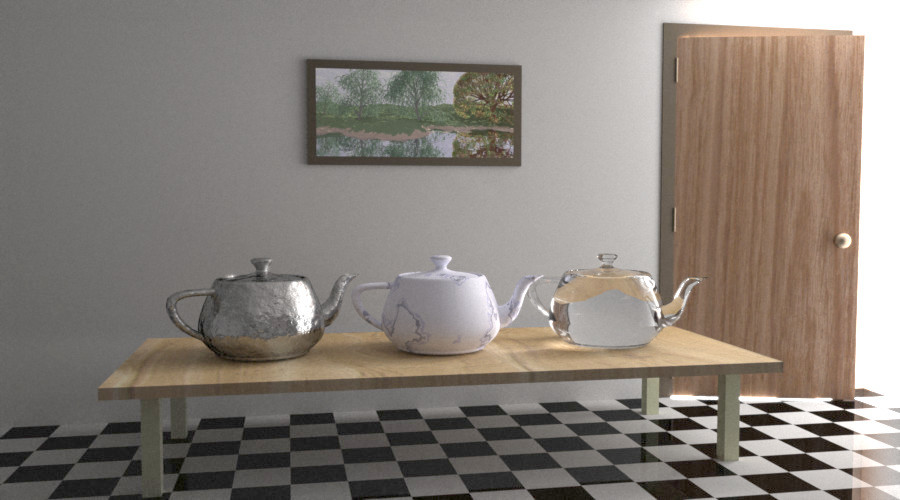
\includegraphics[width=0.7\linewidth]{./mlt.jpg}
    \caption[Metropolis Light Transport]{A scene rendered by the \emph{Metropolis Light Transport} algorithm. Image courtesy of Eric Veach and Leonidas J. Guibas.}
  \label{fig:MLT}
\end{figure}

When the scene and lights therein are static, radiance or irradiance at surface points can be pre-computed and \emph{baked} into a representation which is then efficient to query at real-time. Most commonly, summed irradiance is stored in special images called \emph{Lightmaps} \cite{lightmaps} which are then mapped onto surface geometry. While some implementations \cite{Chen08Halo3} allow directional effects to be captured by encoding the irradiance in an angle-dependent way, dynamic lights and dynamic scene elements must be handled differently. It is common practice to store static parts of the radiance transfer in such a pre-computed representation and add simpler, dynamically computed elements at run-time. Further discussion of static methods is beyond the scope of this thesis, so from now on, it will only be concerned with the dynamic component and assume that any static components are a part of the emissive term.

For the purposes of real-time rendering in games and other interactive three-dimensional applications, the rendering equation is often approximated by replacing the hemispherical integral $\int_\Omega \ldots d \overrightarrow{\omega}'$ with a sum over a finite set of point lights \cite{Naty06Reflectance}:
\[
L_o(\mathbf x, \overrightarrow{\omega}, \lambda) = L_e(\mathbf x, \overrightarrow{\omega}, \lambda) + \sum_l f_r(\mathbf x, \overrightarrow{\omega}', \overrightarrow{\omega}, \lambda) \frac{I_l}{d_l^2} (-\overrightarrow{\omega}' \cdot \overrightarrow{\mathbf n})
\]
where $I_l$ is light intensity and $d_l$ is distance to light $l$ from point $\mathbf x$.

A key factor in the formulae described above is the $f_r$ function. It is called the \emph{bidirectional reflectance distribution function (\textbf{BRDF})} \cite{Nicodemus:65}. It defines how a surface reflects light at a particular position and therefore is the most important element describing the appearance of surfaces in a scene.

\begin{figure}[h!]
  \centering
    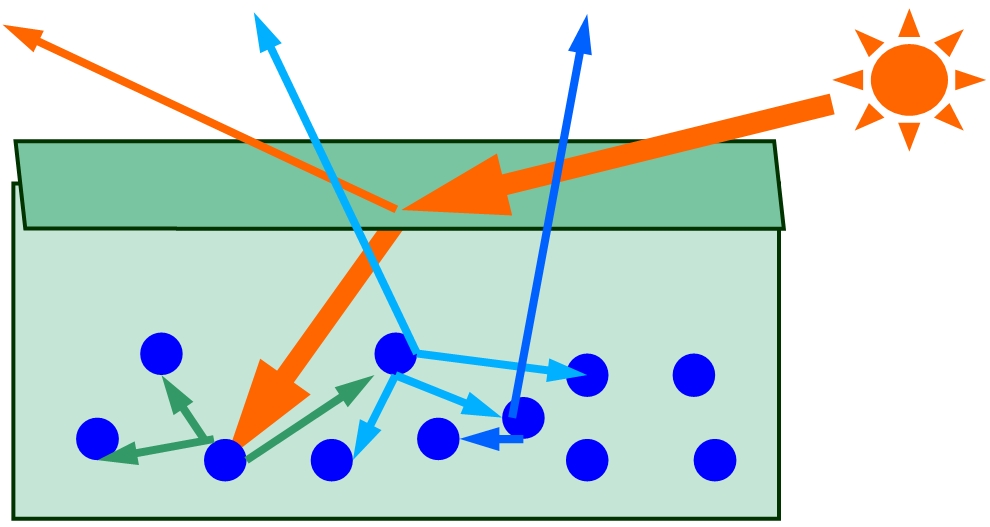
\includegraphics[width=0.4\linewidth]{./Chapters/InhomogeneousDielectric.png}
    \caption[Inhomogeneous dielectric]{Some of the possible light interaction paths within an inhomogeneous dielectric. Image courtesy of Nathaniel Hoffman.}
  \label{fig:InhomogeneousDielectric}
\end{figure}
% TODO: more pictures?

A spatially-varying \emph{BRDF} can describe the complete appearance of a surface including its texture, reflectivity, glossiness, etc. While it is possible to encode this data within a scene representation, it is not practical for most applications due to storage space and memory bandwidth constraints. Simulating light interaction in a precise manner, even under a geometric optics approximation, is very complicated -- for example, Figure \ref{fig:InhomogeneousDielectric} shows some of the possible paths photons might take within an inhomogeneous dielectric. For these reasons, physically and empirically-inspired mathematical models have been proposed, which aim to approximate idealized surfaces of various properties or just provide intuitive parameters to control the appearance of objects. Example models include:
\begin{itemize}
\item Lambertian, describing the idealized diffuser. It is a constant \emph{BRDF}.
\item Phong \cite{Phong}, the first to introduce specular highlights.
\item Cook-Torrance \cite{CookTorrance}, a general model based on \emph{microfacet theory} aimed at rough surfaces, in particular plastics and metals.
\item Ashikhmin-Shirley \cite{Ashikhmin00ananisotropic}, designed to be similar to Phong, but physically plausible, energy-conserving and with intuitive parameters.
\item ABC and ABg \cite{opticalScattering}, able to model light reflection off surfaces with fractal height autocorrelation.
\end{itemize}

\begin{figure}[h!]
  \centering
  \subfigure[Lambertian]{\label{fig:Buddha_Lambert}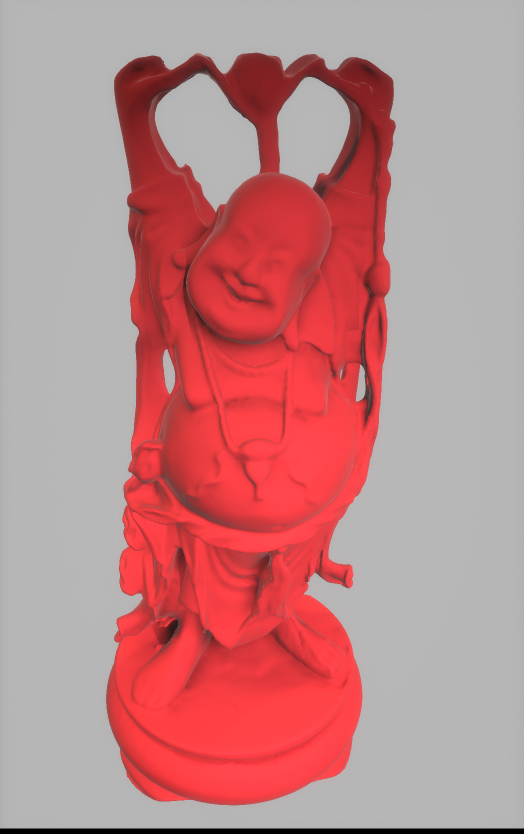
\includegraphics[width=0.32\linewidth]{./BRDFs/Lambert.jpg}}
  \subfigure[Blinn-Phong]{\label{fig:Buddha_BlinnPhong}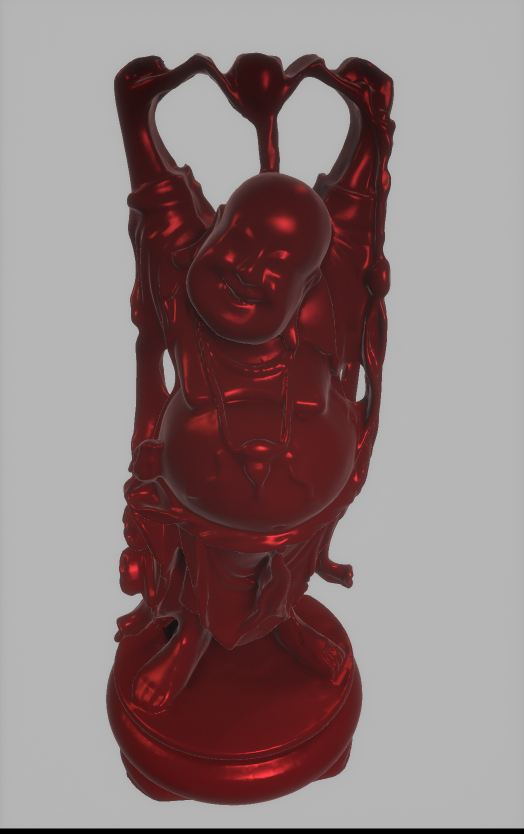
\includegraphics[width=0.32\linewidth]{./BRDFs/BlinnPhong_120.jpg}}
  \subfigure[Ashikhmin-Shirley]{\label{fig:Buddha_AS}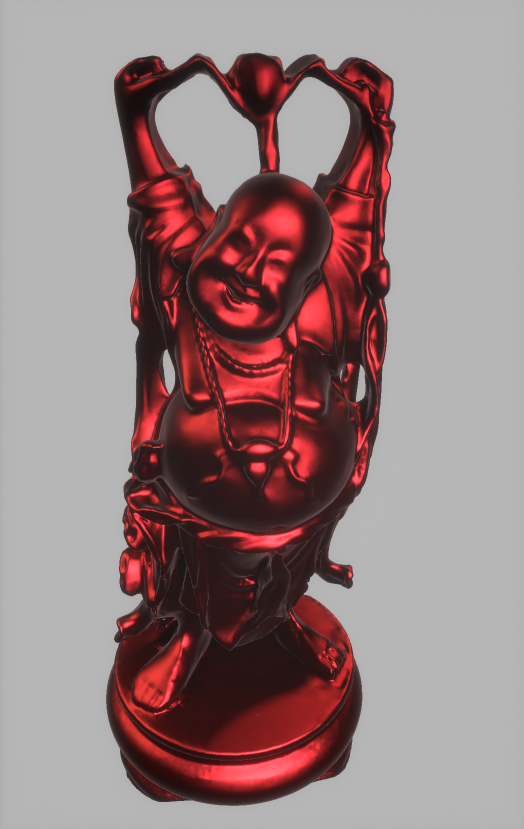
\includegraphics[width=0.32\linewidth]{./BRDFs/AS_f9_r1.jpg}}
\subfigure[Cook-Torrance]{\label{fig:Buddha_CT}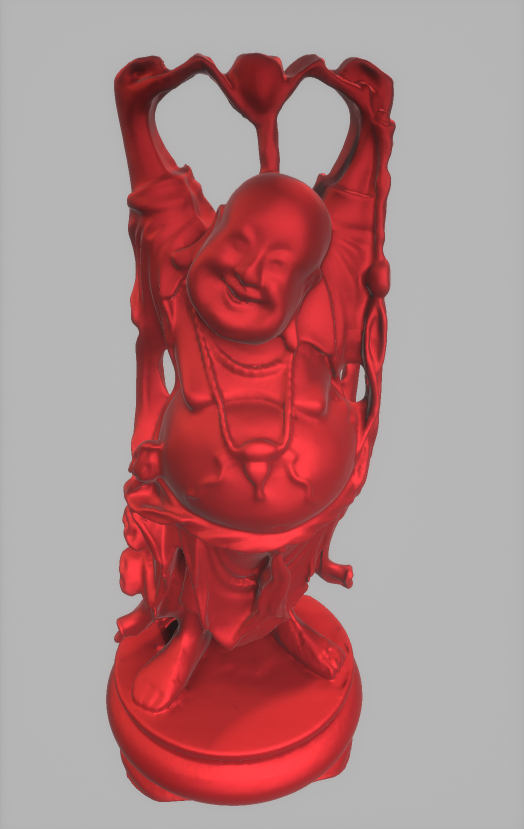
\includegraphics[width=0.32\linewidth]{./BRDFs/CookTorrance_f4_r9.jpg}}
\subfigure[Area ABC]{\label{fig:Buddha_ABC_area}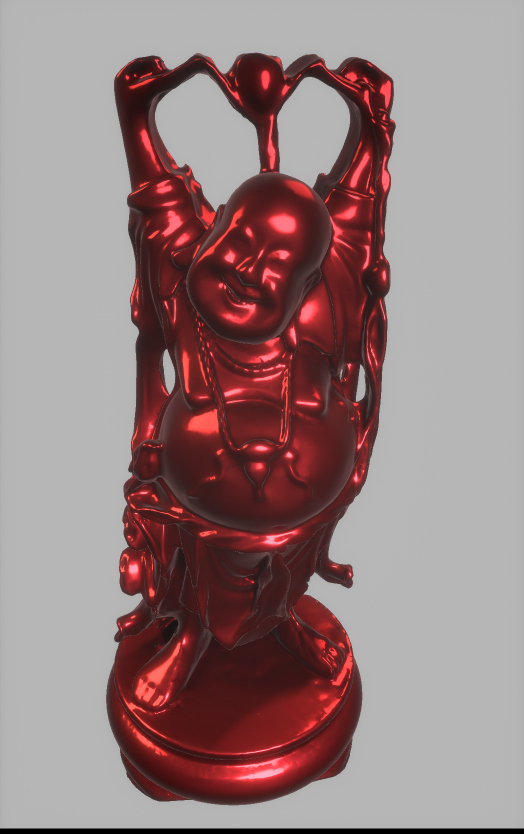
\includegraphics[width=0.32\linewidth]{./BRDFs/ABC_area_approx_b100_c99.jpg}}
\subfigure[ABg]{\label{fig:Buddha_ABg}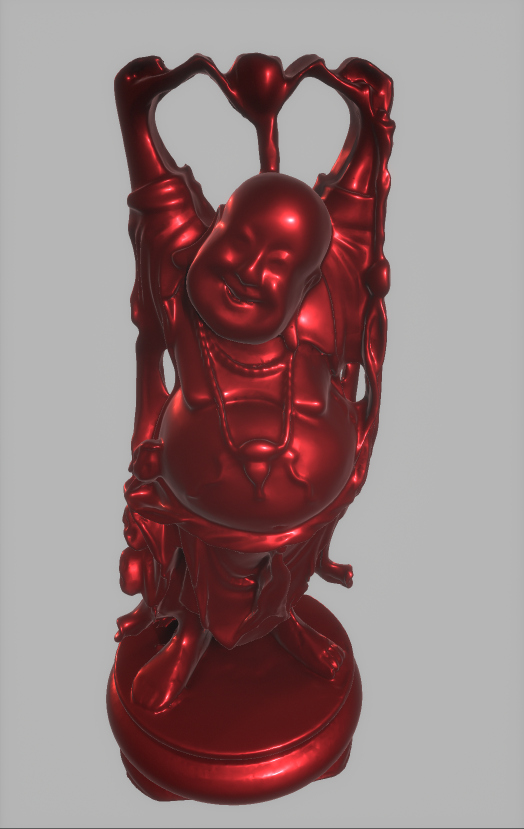
\includegraphics[width=0.32\linewidth]{./BRDFs/ABg_A06_B01_g19.jpg}}
  \caption{Effects of various reflection models on surface appearance. ``Happy Buddha'' model courtesy of The Stanford 3D Scanning Repository.}
  \label{fig:Buddha_reflectionModels}
\end{figure}

In order to introduce details into surfaces, the parameters to light reflection models can be made spatially-varying. For example, the Cook-Torrance model has a \emph{roughness} parameter which defines the width of specular highlights.  Finally, most BRDF models are parametrized with values by which components of the reflection should be scaled -- commonly one parameter for diffuse and one for specular reflectance.

The parameters influencing particular components of the reflection are intuitively called ``colors''. Even though the rendering equation is defined in terms of wavelengths and should be integrated over the entire visible spectrum, real-time computer graphics usually only concerns itself with light transport of three discrete bands. Due to practical considerations, the bands are the red, green and blue components of the \emph{sRGB} color space. Therefore any radiance calculations may be thought to operate on \emph{RGB} triplets, dubbed ``colors'' for the sake of simplicity.

\section{Rasterization}

Real-time rendering requires scenes to be described in a manner which is efficient in terms of storage and interpretation at run-time. Most commonly, objects are discretized as polygonal meshes with extra detail added in by two-dimensional images (called \textbf{textures}) parametrized onto the meshes. The former provide the macro structure of an object, whereas the latter cheaply represent fine detail wrapped over the mesh.

\begin{figure}[h!]
  \centering
  \subfigure{\label{fig:PostApCarWireframe}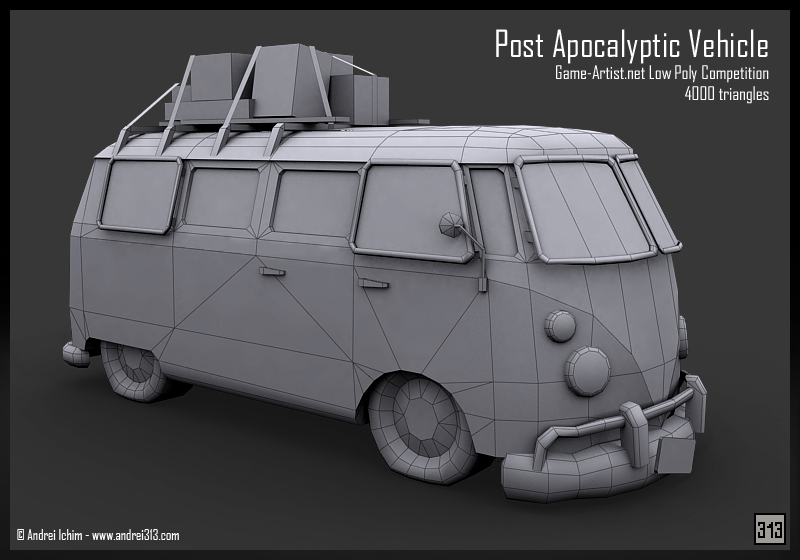
\includegraphics[width=0.45\linewidth]{./Figures/postApocalypticCar/wireframe.jpg}}
  \subfigure{\label{fig:PostApCarTextured}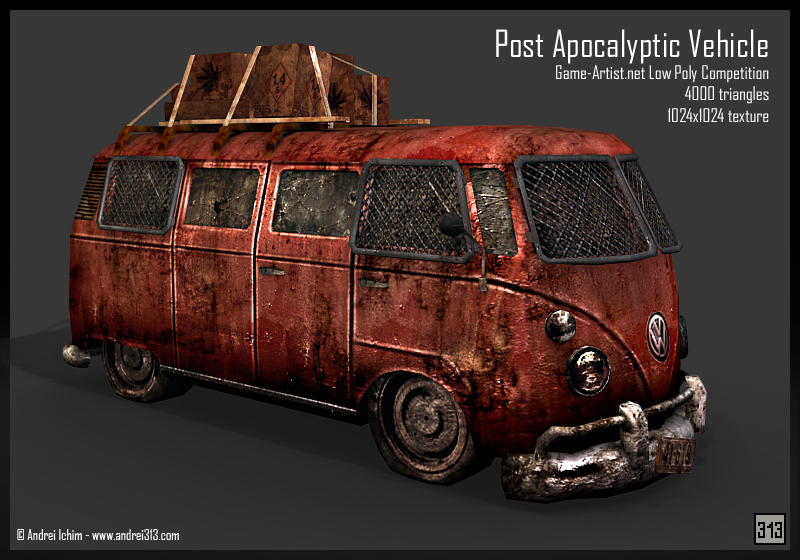
\includegraphics[width=0.45\linewidth]{./Figures/postApocalypticCar/textured.jpg}}
  \caption{The macro- and micro-structure of an object encoded within a triangular mesh mapped with a texture. Images courtesy of Andrei Ichim}
  \label{fig:PostApCar}
\end{figure}

Such a vector-based representation may be visualized on a two-dimensional screen via the \emph{rasterization} algorithm. It is a \emph{forward} rendering algorithm (compared to \emph{backward} methods such as \emph{ray-tracing}) which starts from the scene primitives and via successive transformations, generates colors for the image. The major steps of the algorithm are:
\begin{enumerate}
\item \textbf{Transform} scene geometry into the coordinate space of the viewer.
\item Geometrically \textbf{clip} primitives to the viewable area in order to speed up the next stages and make sure no artifacts are produced.
\item \textbf{Scan-convert} primitives to pixels, calculate their colors and write into the target buffer.
\end{enumerate}
Variations of this algorithm have been used in real-time rendering applications since the beginning of computer graphics because it is simple and scales reasonably well with increasing scene complexity. Thanks to these traits combined with high demand for efficient and detailed rendering, rasterization has found its way into specialized hardware, and finally got integrated into display adapters.

Nowadays every desktop computer system, laptop and recently -- cellphone, contains a graphics card with a highly efficient implementation of the rasterization algorithm, capable of drawing millions of triangles per second, with high-end solutions delivering in excess of a billion triangles per second.

\section{Shading}

%TODO: comma?
Initially, hardware implementations of the rasterization algorithm were very constrained in terms of their functionality. Through a specialized API, such as \textbf{OpenGL} or \textbf{Direct3D}, the programmer could specify a set of textures to be mapped onto geometry, lights to influence it, and the actual geometrical data, which had to be transformed on the CPU side. The graphics card would then perform rendering computations according to a \emph{fixed-function pipeline}, combining the assigned textures in one of a few pre-specified ways, determining how lights influence geometry and perhaps applying a few other, rigid algorithms, such as fog simulation.

Such an approach was initially simple to implement in hardware, but as requirements in display fidelity rose, the number of custom algorithms designed to alleviate constraints of earlier custom algorithms skyrocketed. This resulted in messy APIs, unstable drivers, expensive hardware manufacturing and cumbersome programming against it. Gradually, \emph{programmable shading} was born.

The rasterization algorithm employed by current graphics cards is extensible through the use of programs which operate in various parts of its pipeline. \emph{Shaders} (as that is how they came to be known) provide a means of customizing the rendering, while still staying within the massively parallel implementation of the rasterization algorithm, as employed by GPUs \emph{(Graphics Processing Units)}. They are allowed to influence specific parts of the pipeline, therefore exist in several types. Each type, or \emph{domain} performs computations without referring to the other, in a strictly streamlined order. In case of hardware compliant with \emph{OpenGL 3.2} and \emph{Direct3D 10}, the shader types are \cite{glspec32, SM4}:
\begin{itemize}
\item \textbf{Vertex shaders} -- Execute for every vertex of the input provided to the GPU, they must provide positions of the vertex to be used in scan-conversion of primitives. Normally used to transform the input mesh from a local coordinate system into the space of the viewer, and then (normally through perspective or orthogonal projection) into a special homogeneous basis known as \emph{clip space}. Vertex shaders are a natural fit for deformation algorithms which do not require connectivity information, e.g. \emph{skinning} to make tissue and cloth move in accordance with a hidden skeleton of an articulated character. Another common use is image-based offsetting of vertices of a tessellated grid in order to render height-mapped terrain. Finally, vertex shader must produce all attributes which the next shader in the pipeline might require.
\item \textbf{Geometry shaders} -- An optional part of the rendering pipeline -- if enabled, resides between vertex and fragment processing. Whereas vertex shader operate on individual vertices of the input mesh and produce single vertices in a one-to-one mapping, geometry shaders run post \emph{primitive assembly} and operate on multiple vertices at a time, as well as on optional connectivity information. Moreover, they may output more (or fewer) than a single primitive, therefore being less constrained compared to vertex shaders. A geometry program might, for example, take a single triangle as an input, then subdivide it using a non-linear interpolation scheme and output multiple triangles. Or it might take a point and generate a polygon in its place.
\item \textbf{Fragment shaders} -- Also known as \textbf{pixel shaders}, they work on attributes interpolated from the output of vertex or geometry shaders. Executed for every pixel of the rasterized primitive, they compute the final color of the object, therefore usually performing \emph{texture mapping} and lighting computations.
\end{itemize}

When programmable shading was being introduced, the only way to perform it was by authoring assembly code to run on the GPU. It was also heavily constrained in terms of the number of instructions, registers and attributes it might use. With advancements in GPU technology, the limitations have been largely lifted or at least greatly reduced, e.g. allowing unlimited number of instructions to be evaluated per shader invocation. Several high-level specialized programming languages have also emerged, with the \emph{C}-like \emph{HLSL}, \emph{Cg} and \emph{GLSL} currently leading the pack.

%TODO(?): Say how changing shaders carries a cost, so we can't go wild. Also something about batching.

\section{Mental and hardware programming model mismatch}

Modern GPUs provide a very efficient model of computation allowing for creation of photorealistic renderings of three-dimensional scenes. Still, the programming model is not exactly the most intuitive one. The rendering equation does not feature vertex, geometry and fragment shaders either.

If we consider the elements that make up the rendering equation and the commonly used scene representation, then the logical elements emerge automatically. Under the aforementioned assumptions, we would ideally want to work with shader programs which describe:
\begin{itemize}
\item Light emission
\item Deformation and transformation of scene objects at the macro-scale
\item Materials applied to objects
\end{itemize}

Unsurprisingly, this separation of responsibility is used in many rendering systems which do not use the rasterization algorithm or simply do not run on commodity graphics hardware.

In order to use a similar approach, a real-time rendering system needs to transform such shaders into a form which the GPU is able to execute. This can be approached via relatively simple code-snippet composition \cite{Hargreaves04} or more complex approaches, such as programming language translation \cite{mentalMillMetaSL}.
